\documentclass[12pt]{article}

\usepackage{graphicx}
\usepackage{amsmath}
\usepackage{amssymb}
\usepackage{natbib}
\usepackage{amsfonts}
\usepackage{multicol}
\usepackage{float}
\usepackage{oldgerm}
\usepackage{bm}
\usepackage{mathtools}
\usepackage{wrapfig}
\usepackage{fancyhdr}
\usepackage[export]{adjustbox}
\usepackage{xcolor}
\usepackage[shortlabels]{enumitem}

\pagestyle{empty}

\setlength{\headsep}{0.5cm}
\setlength{\oddsidemargin}{-0.5cm}
\setlength{\textwidth}{16.5cm}
\setlength{\textheight}{24cm}
\voffset = -2cm


\pagestyle{fancy}
\fancyhf{}
\rfoot{
\includegraphics[width=1.0in]{cnm.png}}
\lfoot{ENGR2910 - Midterm 2}
\setlength\parindent{0pt}
\begin{document}

\begin{center}
\hfil
{\large\bf {ENGR 2910-101: Circuit Analysis}}
\hfill Instructor: Brian Rashap\\
Midterm 2  \hfill \\
\hrulefill\\
\end{center}

{\bf Question 1} [25]

Short Answer Responses:
\begin{enumerate}
\item State Ohm's Law in words

\vspace{1cm}

\item What is the equation for Ohm's Law

\vspace{1cm}

\item State Kirchhoff's Current Law (KCL) in words

\vspace{1cm}

\item What is the equation for KCL?

\vspace{1cm}

\item State Kirchhoff's Voltage Law (KVL) in words

\vspace{1cm}

\item What is the equation for KVL?

\vspace{1cm}

\item What are the three Ideal Op Amp assumptions (in words)

\vspace{3cm}

\item What two equations from these assumptions allow us to analyze an Ideal Op Amp?

\vspace{1cm}


\end{enumerate}

\newpage
{\bf Question 2} [25]
\newline

Assuming the Op Amp in the circuit below is ideal:

\begin{figure}[h!]
\centering 
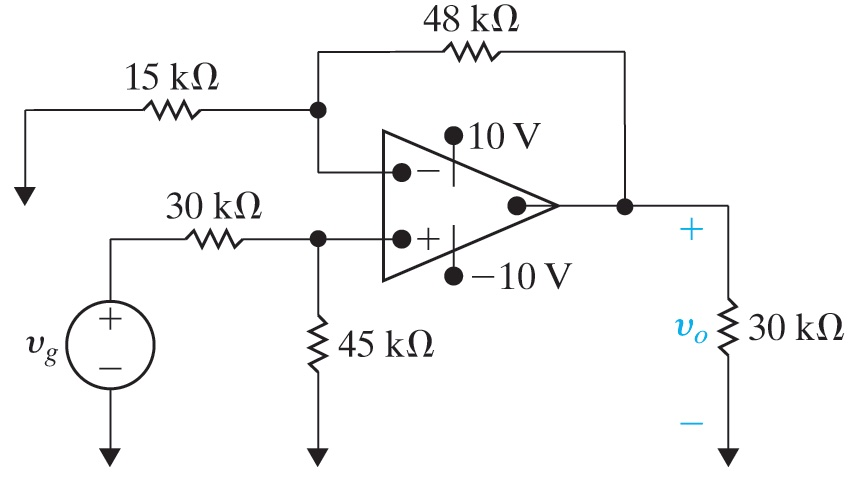
\includegraphics[clip,width=0.49\textwidth]{p05_20.jpg}
\end{figure}

\begin{enumerate}[(a)]
\item What type of Op Amp circuit is this?
\item Calculate $v_0$ when $v_g = 3V$.
\item Specify the range of $v_g$ where the Op Amp operates in the linear region
\item Assume that $v_g$ is set to $5V$ and that the $48 \Omega$ resistor is replaced with a variable resistor. At what value for the variable resistor with the Op Amp first saturate. 
\end{enumerate}

\newpage
{\bf Question 3} [25] 
\newline
The switch in the circuit below has been in Position 1 for a long time. At $t = 0$, the switch moves instantaneously to Position 2. Find $v_0 (t)$ for $t \geq 0^+$.

\begin{figure}[h!]
  \centering 
 \vspace{-0.1in}
 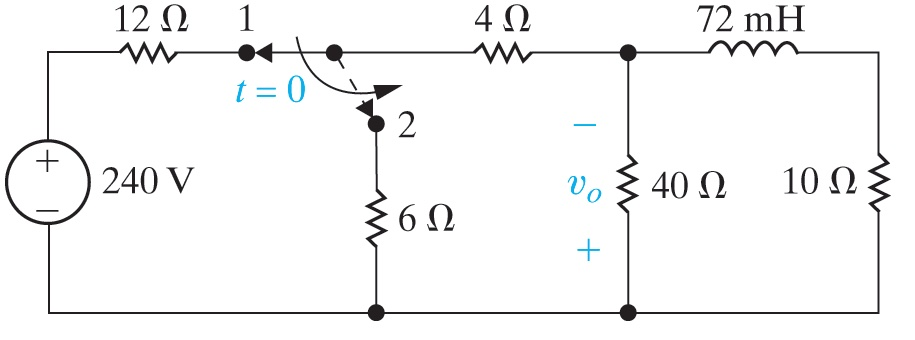
\includegraphics[clip,width=0.64\textwidth]{p07_05.jpg}
\vspace{-0.1in}
\end{figure}


\newpage
{\bf Question 4} [25] 
\newline
For the below circuit has been in position a for a long time. 

\begin{figure}[h!]
     \centering
       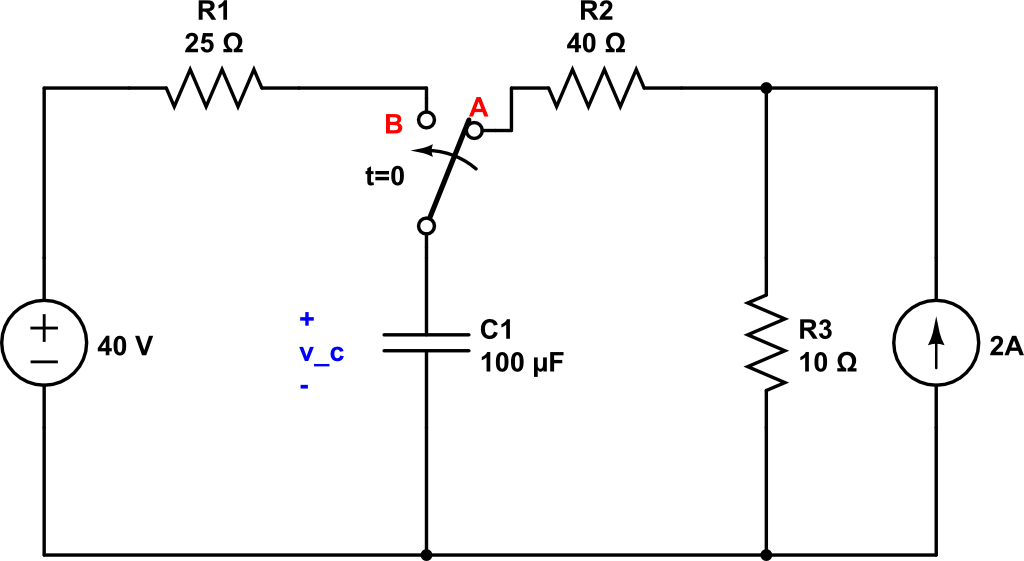
\includegraphics[clip,width=0.6\textwidth]{mid2_3.png}
\end{figure}

\begin{enumerate}[(a)]
\item At $t=0$, the switch instantly moves to position b and stays there. Find:
\begin{enumerate}[(i)]
\item The initial and final values for the capacitor voltage
\item The time constant
\item The expression for the capacitor voltage for $t \geq 0$.
\end{enumerate}
\item At $t = 5ms$ the switch moves back to position a. Find:
\begin{enumerate}[(i)]
\item The initial and final values for the capacitor voltage
\item The time constant
\item The expression for the capacitor voltage for $t \geq 5 ms$.
\end{enumerate}

\end{enumerate}

\end{document}
